% !TeX root = ../../libro.tex
% !TeX encoding = utf8

% TODO -- Lista de TODO's:
%
% - [ ] Escribir la sección de motivación
% - [ ] ? Quitar secciones en la parte del estado del arte, hacerlo todo en conjunto. Quitar seccion de conclusiones en el estado del arte
% - [ ] ? Formateo de las citas

\chapter{Introducción} \label{ich:introduccion}

Las \textbf{ideas principales} de este trabajo son dos. En primer lugar, resolver un problema de \textbf{reconocimiento facial invariante a cambios en la edad}, por sus siglas en inglés, \entrecomillado{AIFR}. Dentro de este problema, nos centraremos en resolver una tarea de \textbf{retrieval}. En segundo lugar, introducir una nueva técnica de aprendizaje automático, que busca \textbf{solucionar los principales problemas que plantea el uso de la función de pérdida \entrecomillado{triplet loss}} \cite{informatica:principal}. Esta técnica introduce una forma de generar los \textit{batches} de triples de forma \textit{online}. Esto evita tener un paso separado en el ciclo de entrenamiento, dedicado únicamente a volver a generar de forma \textit{offline} nuevos \textit{batches} de triples. Y de paso, se consigue normalizar la dificultad que suponen estos conjuntos de triples. Estudiaremos esta técnica detalladamente en \customref{isec:batching}.

Esta situación plantea una serie de \textbf{problemas}:

\begin{itemize}
    \item La nueva técnica que busca mejorar el uso de \textit{Triplet Loss} se plantea en un \textbf{ambiente completamente distinto} al de \textit{AIFR}, en concreto, en el ámbito de re-identificación de personas \cite{informatica:principal}
        \begin{itemize}
            \item En el problema de re-identificación de personas se trabaja normalmente con imágenes de cuerpo completo y con diferencias temporales entre imágenes muy acotadas. La tarea es seguir identificando con la misma identidad a una persona que ha desaparecido momentáneamente de la escena.
            \item Mientras que los problemas principales en \textit{AIFR} son otros (y se detallarán en \customref{ich:descrp_problema}). Buscamos asignar la misma identidad a imágenes faciales de una persona, tomadas en momentos muy distintos de su vida.
            \item Por tanto, no disponemos de literatura en la que se expongan resultados obtenidos de aplicar estas técnicas a nuestro ámbito de trabajo
        \end{itemize}
    \item Como veremos en \customref{ich:estado_arte}, no hay trabajos previos que hayan aplicado \textit{triplet loss} (y mucho menos la variación que introducimos) para resolver un problema de \textit{AIFR}. Por tanto, el acceso a literatura es todavía más restringido
    \item Esta técnica cambia fundamentalmente la forma de generar \textit{batches} de datos. Y por tanto, modifica en esencia muchas partes primarias del proceso de aprendizaje. Por ejemplo, el ciclo de entrenamiento, el cálculo de métricas durante el entrenamiento, el acceso a los datos... Es por este motivo que hemos tenido que realizar \textbf{implementaciones personalizadas de casi todos estos elementos}, sin poder hacer uso de la mayoría de implementaciones que ofrecen las librerías de aprendizaje automático. Esto supone que deberemos dedicar \textbf{mucho más tiempo del esperado a la implementación}, teniendo en cuenta que hay que prestar \textbf{especial atención a la optimización y validación} mediante \textit{tests} de estos nuevos módulos. Esto se plasma en \customref{ich:implementacion}
    \item Como comentaremos en \customref{ich:conclusiones}, este trabajo \textbf{no ha dado buenos resultados en la práctica}, comparado con otras técnicas más establecidas en el ámbito del \textit{AIFR}. Sin literatura que aplique nuestras nuevas técnicas en nuestro ámbito, como veremos en \customref{isec:interesareaestudio}, tenemos que \textbf{basarnos únicamente en todo el trabajo realizado para estudiar el por qué} de este mal comportamiento.
\end{itemize}

Aunque entraremos en detalle en \customref{isec:github_buenas_practicas}, todo el desarrollo del código y de la presente memoria se ha relaizado en un repositorio abierto de \textit{Github} \cite{informatica:repogithub}. Aquí se pueden consultar todos los \textit{commits}, \textit{pull requests}, \textit{issues}, \textit{feature branches} y la integración continua con \textit{Github Actions}.

La siguiente imagen ayuda a entender la diferencia entre el problema de re-identificación (ambiente en el que se introduce la mejora de \textit{triplet loss} que vamos a explorar) y el problema de \textit{AIFR}:

\begin{figure}[H]
    \centering
    \ajustarsubcaptions
    \begin{subfigure}{0.4\textwidth}
        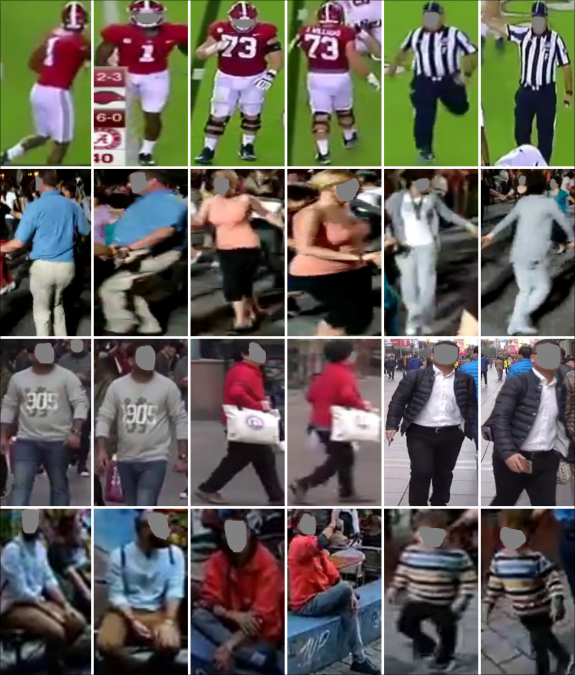
\includegraphics[width=0.9\textwidth]{informatica/ejemplo_reid}
        \caption{Ejemplo de un problema de re-identificación. Imágenes del \textit{dataset} \textit{LuPerson}. Imagen extraída de \cite{informatica:luperson}}
    \end{subfigure}%
    \begin{subfigure}{0.6\textwidth}
        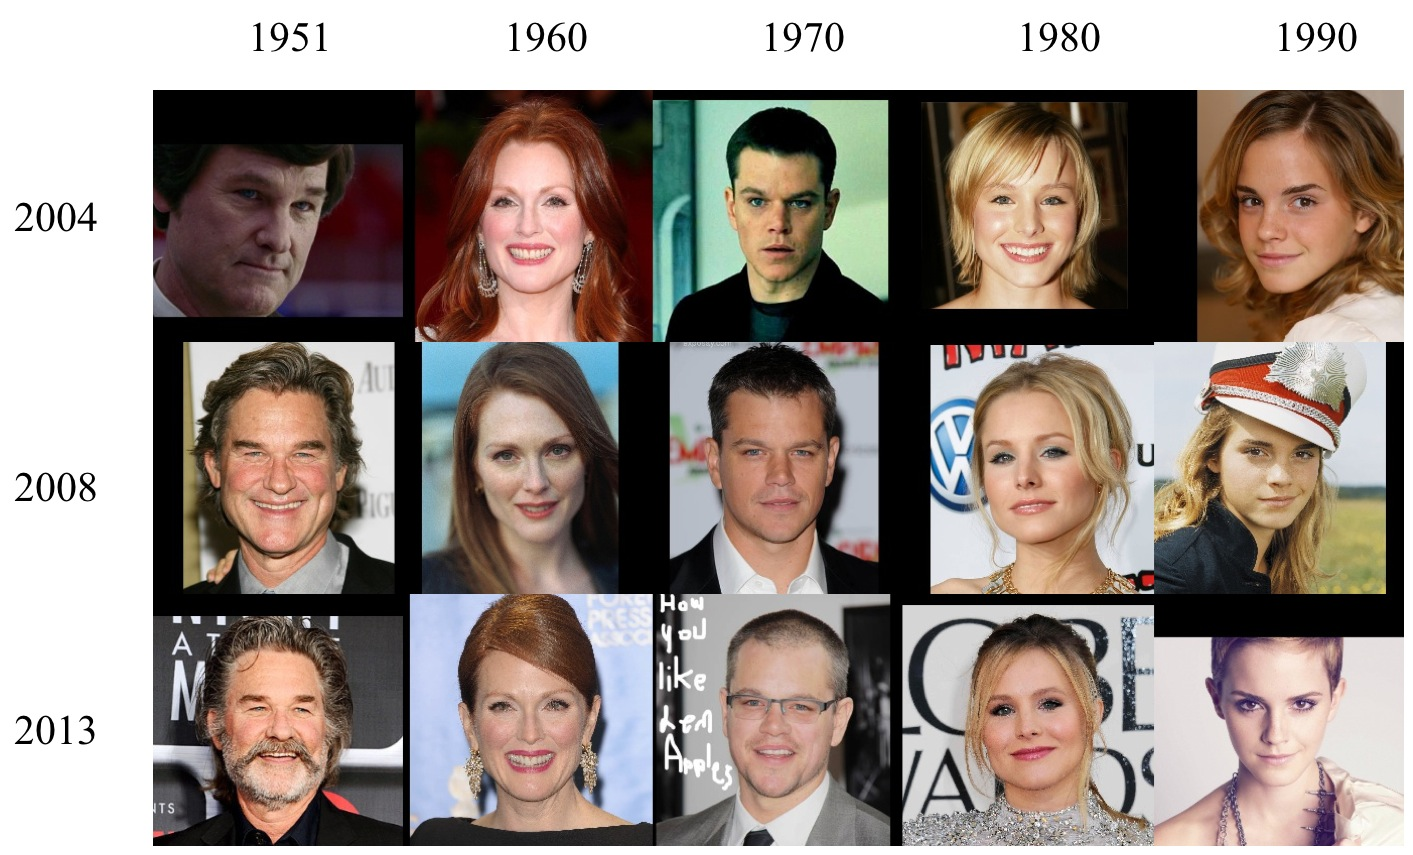
\includegraphics[width=0.9\textwidth]{informatica/cacd_example}
        \caption{Ejemplo de un problema de \textit{AIFR}. Imágenes del \textit{dataset} \textit{CACD}. Imagen extraída de \cite{informatica:paper_cacd}}
    \end{subfigure}

    \caption{En el ejemplo de re-identificación podemos observar pares de imágenes, de cuerpo completo, de una persona en dos instantes de tiempo muy cercanos (misma ropa, prácticamente el mismo fondo). Además, en ese ejemplo el \textit{dataset} borra información sobre el rostro de las personas. En el ejemplo de \textit{AIFR}, podemos ver varias imágenes de una persona en distintos momentos de su vida, con años de diferencia. Nos centramos en la información de la cara de las personas. La variabilidad se centra en cambios en los rasgos faciales por el paso de los años, no se usa la misma ropa, ...}
\end{figure}

\section{Descripción del problema} \label{ich:descrp_problema}

Como ya se ha comentado, trabajaremos un problema de \textbf{reconocimiento facial invariante a la edad} (\textit{AIFR}, de sus singlas en inglés \entrecomillado{Age-Invariant Face Recognition}), introduciendo una \textbf{variación sobre la función de pérdida \textit{Triplet Loss}} para poder generar triples de forma \textit{online}. En esta sección nos centraremos en presentar el problema \textit{AIFR}, mientra que la nueva técnica de cómputo de la función de pérdida será estudiada en profundidad en \customref{isec:triplet_loss}.

El \textbf{problema de reconocimiento facial invariante a la edad} es el siguiente: dada una imagen de una persona, debemos ser capaces de discriminar entre imágenes de otras personas (negativas) e imágenes de la persona dada en primera instancia (positivas). Todo esto teniendo en cuenta diferencias significativas en la edad de las personas que aparecen, tanto en imágenes negativas como positivas.

Este problema se divide en las siguientes \textbf{subtareas}:

\begin{itemize}
    \item \textbf{\textit{Retrieval}} o búsqueda: dada una imagen de una persona objetivo y una base de datos de imágenes, devolver un número específico de imágenes tomadas de la base de datos de la persona objetivo

        \begin{itemize}
            \item Esta es la tarea que intentamos resolver en el presente trabajo
            \item Un escenario para esta tarea es, por ejemplo, tras la desaparición de una persona, tomar imágenes de distintas bases de datos policiales y estudiar las 100 imágenes con mayor probabilidad de corresponderse con la identidad de la persona desaparecida
            \item A la acción de aportar una imagen, una base de datos, y tomar las $N$ imágenes que son más probables de coincidir en la identidad de la persona de la primera imagen, la llamaremos \textbf{consulta} o \textbf{\textit{query}}. A la imagen pasada como parámetro se le llama \textbf{\textit{key}} o llave.
        \end{itemize}

    \item Verificación: dadas dos imágenes, el modelo debe decidir si se trata de la misma persona o no.
        \begin{itemize}
            \item Un escenario es, por ejemplo, comprobar la imagen del pasaporte y la imagen obtenida de las cámaras de los puestos de control de acceso automático \cite{informatica:docface}
        \end{itemize}

    \item Clasificación: tras entrenar con imágenes asociadas a un grupo de personas, dada una imagen de entrada, tenemos que reconocer la identidad de la persona que aparece en la imagen como una de las identidades usadas durante el entrenamiento
        \begin{itemize}
            \item Esto fuerza a que solo podamos trabajar con un número prefijado de personas, y no con personas arbitrarias que nunca hayamos visto antes. Esta restricción hace que sea la tarea menos interesante (y quizás, la más sencilla de resolver)
            \item Por lo tanto, es inusual encontrar trabajos que usen las técnicas presentadas en este trabajo para intentar resolver este tipo de problemas
        \end{itemize}

\end{itemize}

En consecuencia, nuestra tarea es la de realizar \textit{retrieval} de imágenes faciales invariante a cambios en la edad. En adelante, salvo que induzca a confusión, nos referiremos a esta tarea simplemente como \textit{AIFR}, sin especificar que estamos realizando concretamente \textit{retrieval} y no alguna de las otras subtareas que acabamos de especificar.

La siguiente imagen explica visualmente la tarea de verificación:

\begin{figure}[H]
    \centering
    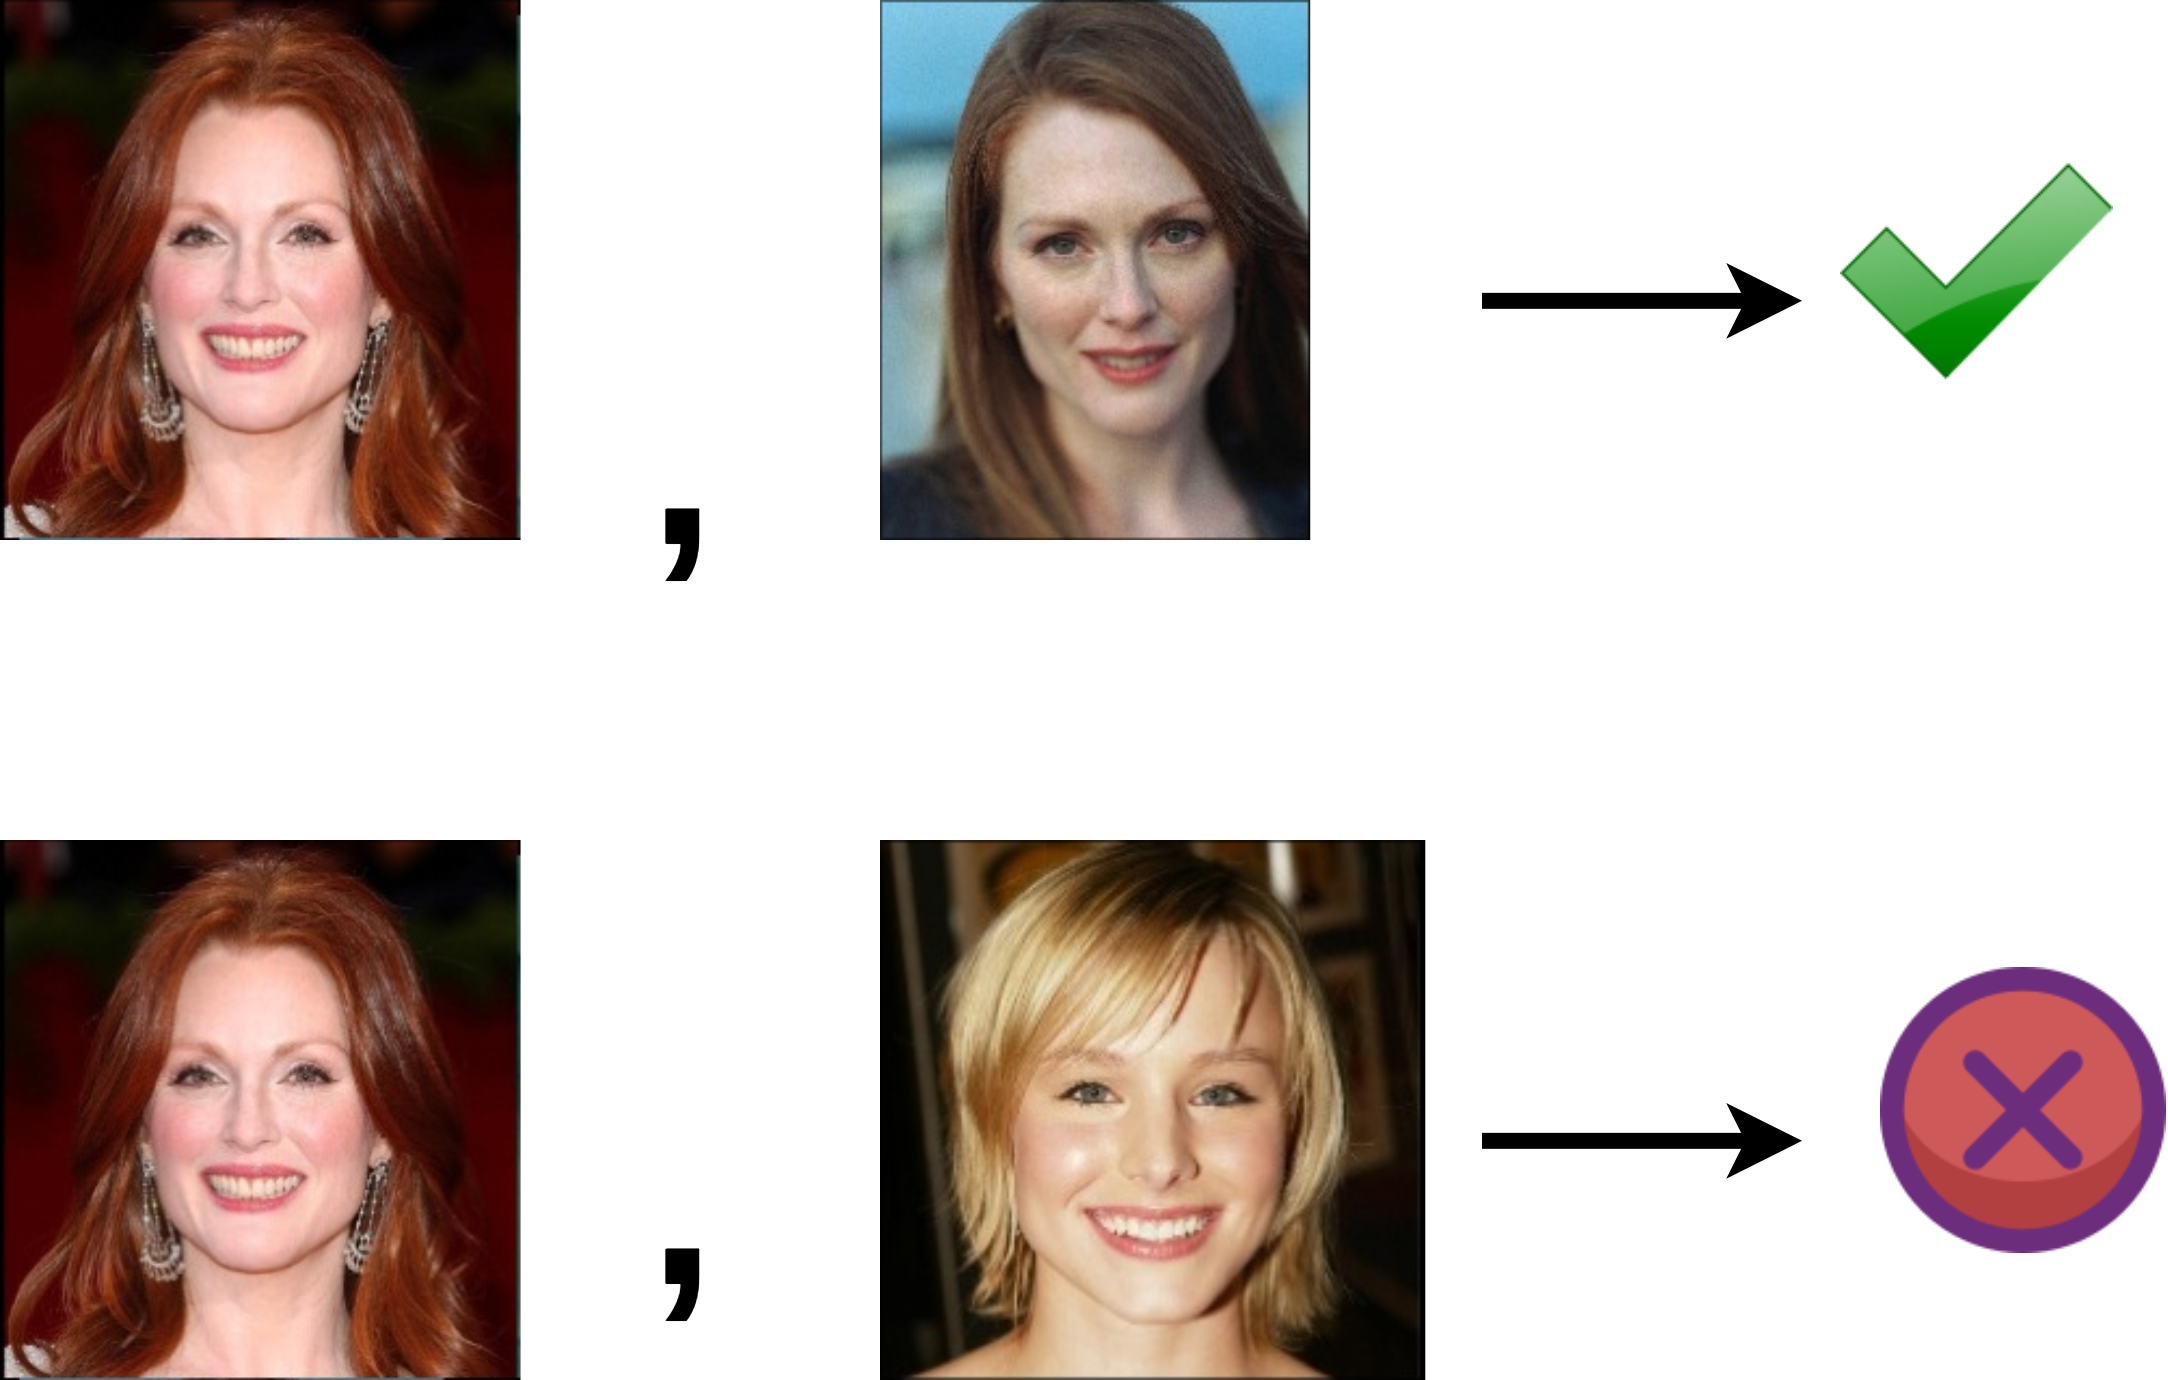
\includegraphics[width=0.9\textwidth]{informatica/ejemplos_tareas/verification}
    \caption{Ejemplo gráfico de la tarea de verificación. Dado un par de imágenes, decidimos si se corresponden a la misma identidad o si son dos personas distintas. Imágenes extraídas de \cite{informatica:cacd_dataset}, diagrama generado con \url{draw.io}}
\end{figure}

Y la siguiente imagen explica visualmente la tarea de \textit{retrieval}:

\begin{figure}[H]
    \centering
    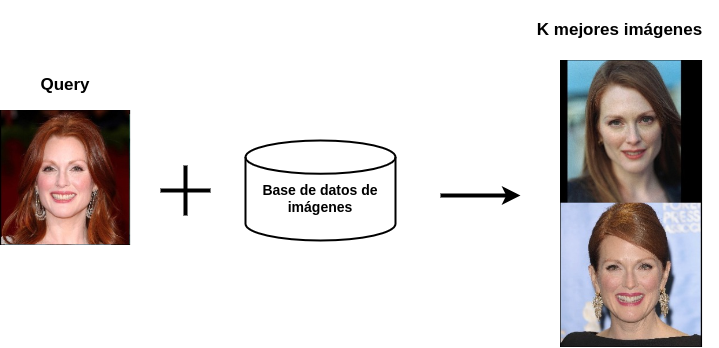
\includegraphics[width=1.0\textwidth]{informatica/ejemplos_tareas/retrieval}
    \caption{Ejemplo gráfico de la tarea de \textit{retrieval}. Dada una imagen objetivo o \textit{query}, y una base de datos de imágenes candidatas, devolvemos las mejores $K = 2$ imágenes. Imágenes extraídas de \cite{informatica:cacd_dataset}, diagrama generado con \url{draw.io}}
\end{figure}

Además de los problemas comunes de la visión por computador, este problema tiene las siguientes \textbf{dificultades específicas} \cite{informatica:challenges_retrieval}:

\begin{itemize}
    \item \textbf{Invarianzas}: en nuestro problema esto es especialmente relevante. Al trabajar con imágenes tomadas en instantes de tiempo muy variados, las características de la imagen pueden variar considerablemente.
        \begin{itemize}
            \item Pensemos, por ejemplo, en fotografías antiguas que fueron tomadas en blanco y negro, en contraste con fotografías más actuales en color
            \item O cambios considerables en características de la cámara con la que se toman las fotografías
        \end{itemize}
    \item \textbf{Distractores}: nuestro modelo se debe centrar en estudiar las caras que aparezcan en la imagen, ignorando otros elementos, como los que puedan aparecer en el fondo
    \item \textbf{Eficiencia}: a la hora de que nuestro modelo reciba una \textit{query}, desconocemos el tamaño de la base de datos sobre la que tenemos que operar. Por tanto, nuestro modelo deberá ser eficiente para poder trabajar con grandes bases de datos sin que el tiempo de respuesta se vea gravemente afectado
    \item Problemas asociados al \textbf{envejecimiento}: cómo varía la cara con el paso de los años es un proceso muy complejo. Algunos de los factores que afectan a este envejecimiento \cite{informatica:tecnica_sintesis_aifr} son:
        \begin{itemize}
            \item Factores intrínsecos como la genética o la etnia
            \item Factores extrínsecos como el ambiente o los hábitos de vida
        \end{itemize}
    Además, algunas características de la cara cambian drásticamente con el paso de los años. Por ejemplo, la textura (aparición de arrugas, lunares, vello, \ldots), cambios en la forma de la cara (cambio en el peso corporal)

\item Tenemos que trabajar con \textbf{identidades que nunca hemos visto} en nuestros datos de entrenamiento. En otras tareas, como por ejemplo la de clasificación de objetos cotidianos, ocurre algo parecido. Por ejemplo, tenemos imágenes de coches que nunca ha visto previamente el modelo. Sin embargo la diferencia radica en que en nuestro problema el modelo debe saber identificar identidades, mientras que en el modelo de clasificación este debe saber identificar categorías

\item Nuestro modelo debe identificar como similares (véase \customref{isec:embeddings}) imágenes de la misma persona, aunque sea en momentos muy distintos. Y debe identificar como no similares imágenes de personas distintas. Es muy fácil que ocurra que dos imágenes de la misma persona tomadas con muchos años de diferencia parezcan más distintas que dos imágenes de dos personas distintas pero de la misma edad. Por ejemplo, esto se puede ver en \customref{img:messi_distintos_otro_adulto}

\item Aunque desarrollemos esto más tarde en \customref{isec:base_datos_usada}, los \textbf{\textit{datasets} de \textit{AIFR} son escasos y presentan problemas} \cite{informatica:tecnica_sintesis_aifr}. Algunas de estas bases de datos son muy pequeñas. Otras, son de un tamaño más grande, pero presentan mucha menos variabilidad en los rangos de edad. Y por supuesto, muchas de estas bases de datos presentan problemas de representatividad (etnia, sexo).
\end{itemize}

\begin{figure}[H]
\centering
    \begin{subfigure}{0.5\textwidth}
        \centering
        \includegraphics[width=0.5\linewidth]{informatica/messi_niño}
        \caption{Edad temprana. Imagen extraída de \cite{informatica:webimg_messi_pequeno}}
        \label{img:messi_pequeno}
    \end{subfigure}%
    \begin{subfigure}{.5\textwidth}
        \centering
        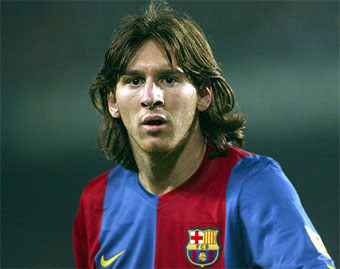
\includegraphics[width=0.8\linewidth]{informatica/messi_joven}
        \caption{Edad joven. Imagen extraída de \cite{informatica:webimg_messi_joven}}
    \end{subfigure}%

    \begin{subfigure}{.5\textwidth}
        \centering
        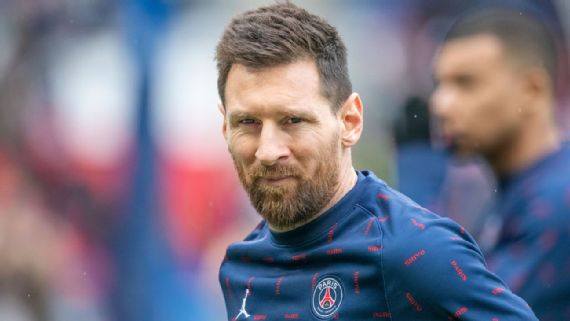
\includegraphics[width=0.6\linewidth]{informatica/messi_adulto}
        \caption{Edad adulta. Imagen extraída de \cite{informatica:webimg_messi_adulto}}
        \label{img:messi_adulto}
    \end{subfigure}%
    \begin{subfigure}{.5\textwidth}
        \centering
        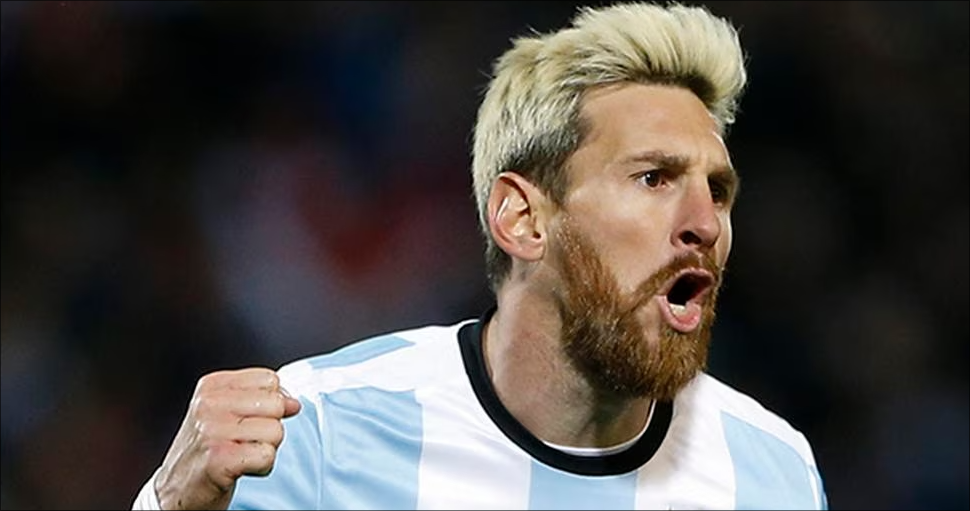
\includegraphics[width=0.8\linewidth]{informatica/messi_rubio}
        \caption{Otra imagen en la edad adulta, pocos años después. Imagen extraída de \cite{informatica:webimg_messi_rubio}}
    \end{subfigure}

    \caption{Lionel Messi en cuatro momentos distintos de su vida}
    \label{img:messi_cuatro_edades}

\end{figure}

Las imágenes presentadas en \customref{img:messi_cuatro_edades} son un buen ejemplo de los problemas específicos que acabamos de comentar. Por ejemplo, en la fotografía \ref{img:messi_adulto} podemos ver que, en el fondo de la imagen, aparece otro jugador, y nuestro modelo podría distraerse por este hecho. La imagen en la que aparece siendo más pequeño, \ref{img:messi_pequeno}, es de una calidad mucho menor que el resto de imágenes. No ha desarrollado todavía rasgos faciales muy característicos. La variabilidad en el estilo de pelo es total. Se puede apreciar perfectamente como el paso de los años va modificando los rasgos de la cara. Y todo esto sin comentar problemas comunes y bien conocidos en la visión por computador, como por ejemplo, cambios en la pose, iluminación, \ldots

Veámos otro ejemplo:

\begin{figure}[H]
\centering
    \begin{subfigure}{0.5\textwidth}
        \centering
        \includegraphics[width=0.6\linewidth]{informatica/messi_niño}
        \caption{Messi en una edad temprana}
    \end{subfigure}%
    \begin{subfigure}{.5\textwidth}
        \centering
        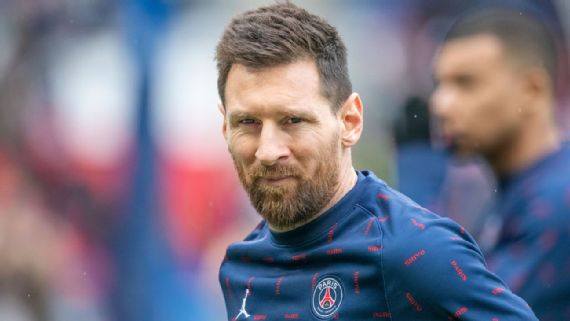
\includegraphics[width=0.8\linewidth]{informatica/messi_adulto}
        \caption{Messi en edad adulta}
    \end{subfigure}

    \begin{subfigure}{.8\textwidth}
        \centering
        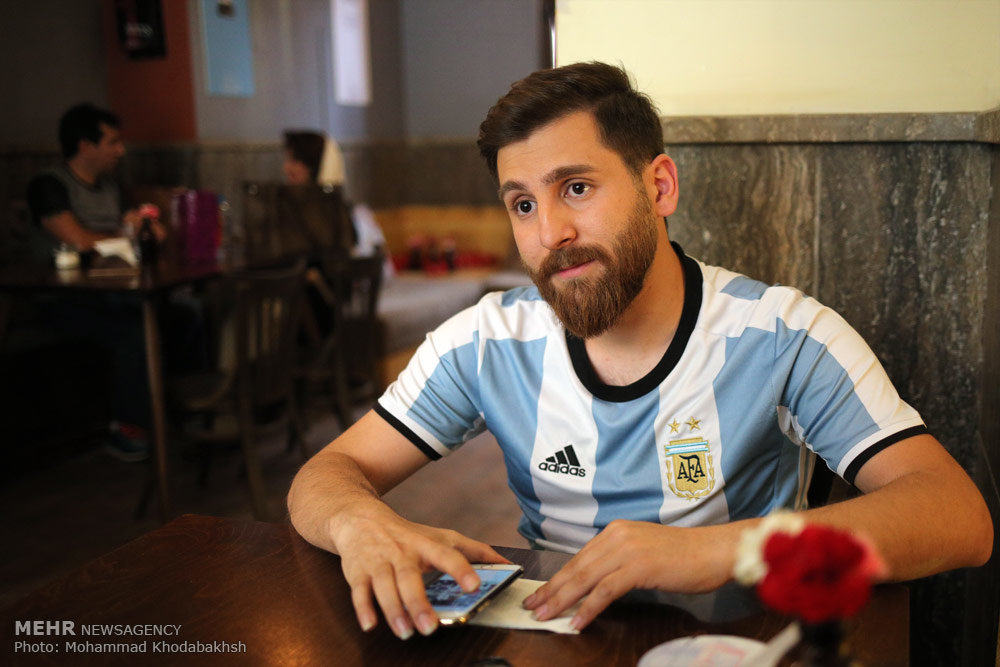
\includegraphics[width=0.6\linewidth]{informatica/doble_messi}
        \caption{Riza Perestes, ciudadano iraní. Imagen extraída de \cite{informatica:imitador_messi}}
    \end{subfigure}

\caption{Lionel Messi en dos momentos distintos de su vida, y Riza Perestes, ciudadano iraní con gran parecido}
\label{img:messi_distintos_otro_adulto}
\end{figure}

En este ejemplo vemos un problema que hemos comentado previamente: tenemos más parecido entre dos personas distintas pero de la misma edad, que entre la misma persona pero a distintas edades. En este caso el parecido es extraordinario, pero es razonable que nuestro modelo tenga dificultades en asignar mayor parecido a imágenes de la misma persona en su adultez y niñez, que a imágenes de dos personas distintas, ambas con barba y mismo corte de pelo, por poner un ejemplo.

Aunque más tarde desarrollemos en profundidad el uso de \textit{triplet loss} (\customref{isec:triplet_loss}), conviene hacer unos pequeños apuntes sobre esta técnica. Para empezar, el uso de esta función de pérdida ya nos indica que, de una forma u otra, nuestra solución al problema va a fundamentarse en el cómputo de un \textit{embedding} (véase \customref{isec:embeddings}).

Gracias a que nuestro modelo aprende un \textit{embedding} semántico, podríamos haber resuelto también alguno de los otros problemas que ya hemos mencionado, por ejemplo, el de verificación. Sin embargo, para acotar el alcance de este trabajo, hemos decidido centrarnos en \textit{retrieval}.

Además, por cómo hemos diseñado el código (véase \customref{isubs:impl_retr_adapter}), la adaptación del modelo a una nueva tarea es inmediata, y en teoría, si el modelo inicial es competente, el modelo adaptado también debería serlo.

Y para finalizar, introducimos los \textbf{dos enfoques principales usados para resolver problemas de \textit{AIFR}}, que estudiaremos en profundidad en \customref{ich:estado_arte}:

\begin{enumerate}
    \item El primer enfoque es aplicar modelos generativos adversarios (\textit{GAN}). Por ejemplo, el \textit{Age Invariant Model} o \textit{AIM} propuesto en \cite{informatica:tecnica_sintesis_aifr}.
    \item El segundo enfoque es directamente trabajar sobre una base de datos que presente la suficiente variabilidad en la edad de los individuos, y desarrollar un modelo que realice nuestra tarea. Este enfoque casi siempre pasa por computar un \textit{embedding}. Este será el enfoque que sigamos.
\end{enumerate}
\todo{\cite{informatica:paper_cacd} habla en la página 3 de \url{http://www.sirius.umiacs.io/papers/chen14tmm.pdf} de las aproximaciones al problema!}

\section{Motivación}

El ámbito de aplicación de un modelo capaz de reconocer caras independientemente de cambios de edad es amplio, destacando el ámbito de la informática forense. Algunos ejemplos de aplicación son:

\begin{itemize}
    \item Reconocer caras de sospechosos que llevan en busca un tiempo en imágenes de videovigilancia
    \item Reconocer caras de personas desaparecidas un tiempo considerable, en imágenes de videovigilancia, controles de aeropuertos, ...
    \item Verificación automática de documentos de identidad en puestos de control \cite{informatica:tecnica_sintesis_aifr}. Por ejemplo, los puestos de control automáticos de aeropuertos. En estos puestos, una máquina verifica que la imagen que aparece en el pasaporte coincida con una imagen tomada en ese momento con una cámara.
    \item Consultar en una base de datos policial las 10 identidades que más se parecen a la imagen de una persona dada
\end{itemize}

Por ejemplo, en 2021 se pusieron en marcha en España máquinas \textit{ABC System} para realizar automáticamente el control de pasaportes en aeropuertos \cite{informatica:articulo_abc_system}. Una de las tareas de esta máquina es la de verificar que la fotografía que aparece en el pasaporte se corresponde con la persona que está intentando pasar el control. Esto se muestra en las siguientes imágenes:

\begin{figure}[H]
    \centering
    \begin{subfigure}{0.4\textwidth}
        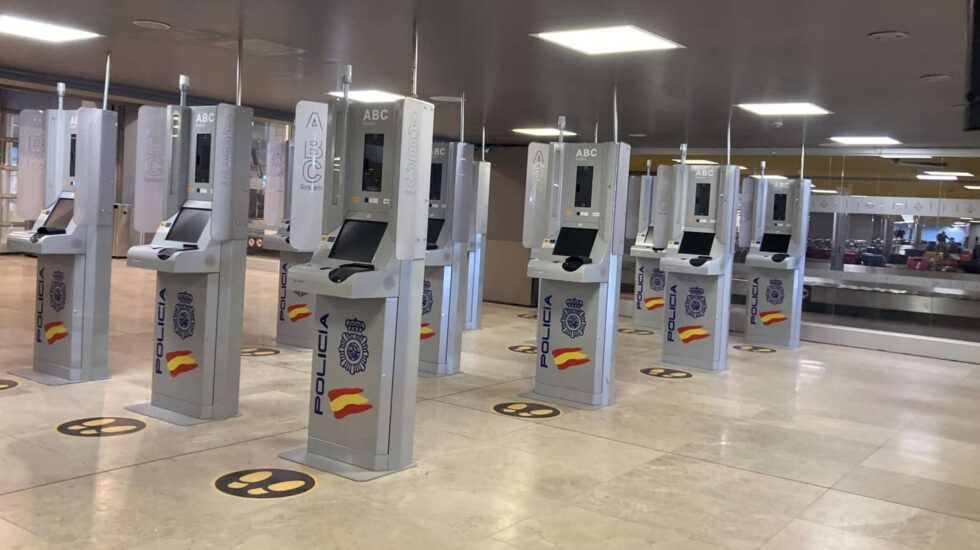
\includegraphics[width=1.0\textwidth]{informatica/ejemplo_abc_system_01}
    \end{subfigure}
    \begin{subfigure}{0.4\textwidth}
        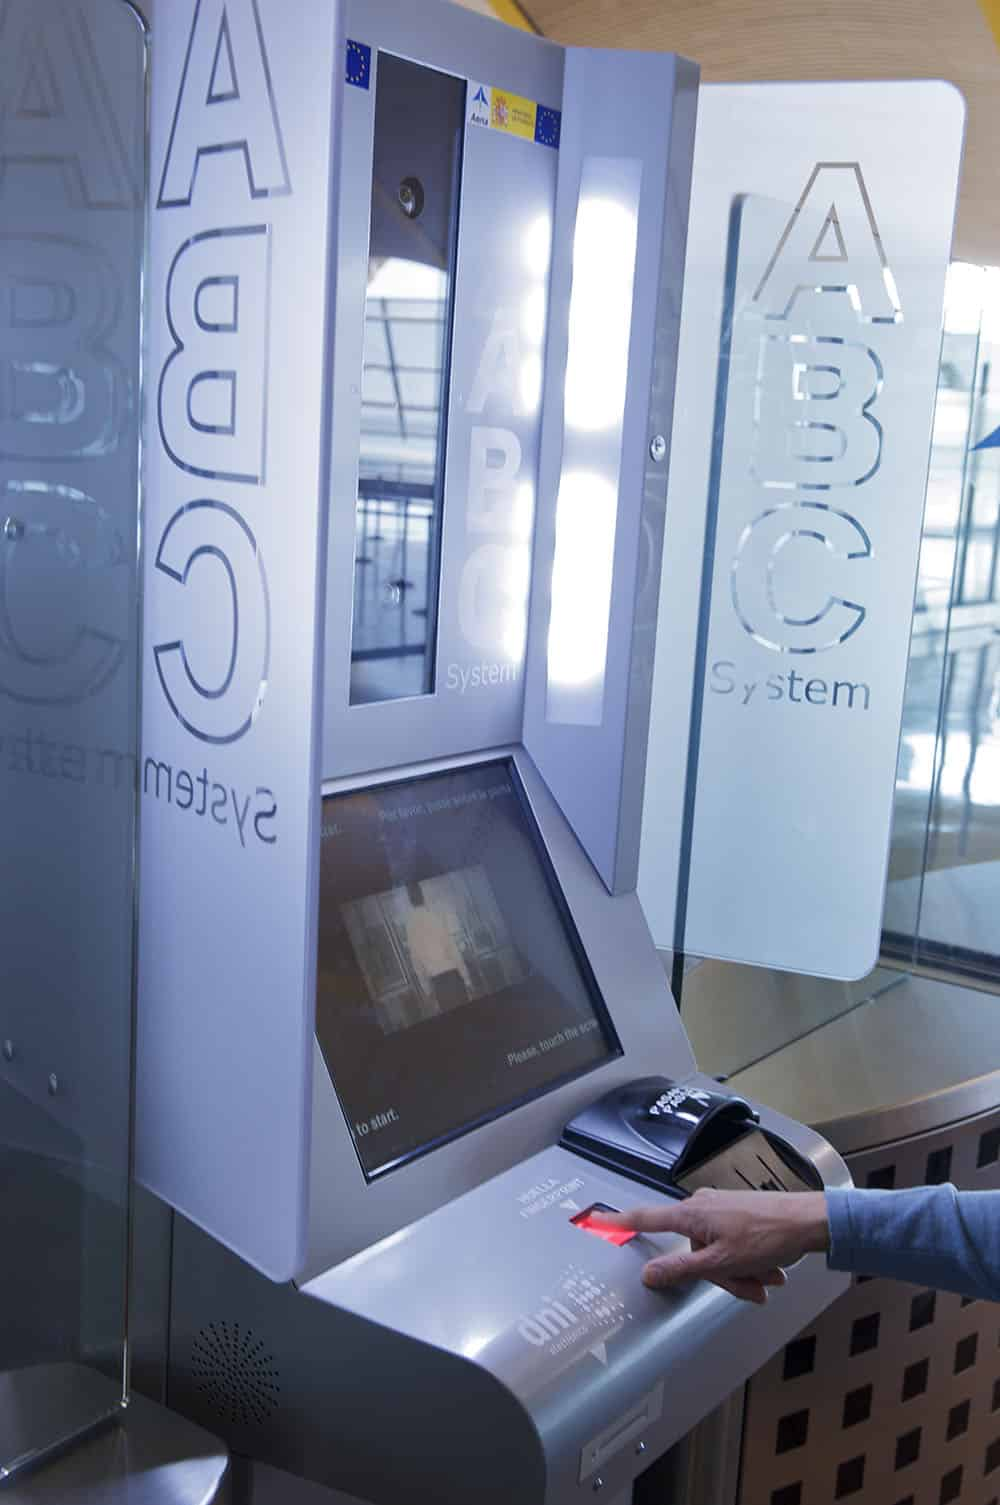
\includegraphics[width=1.0\textwidth]{informatica/ejemplo_abc_system_02}
    \end{subfigure}

    \caption{Máquinas \textit{ABC System} para realizar el control de pasaportes en aeropuertos de forma automática. Entre otras tareas, verifican que la fotografía del pasaporte se corresponda con una imagen tomada por la cámara de la máquina. Imágenes extraídas de \cite{informatica:articulo_abc_system}}
\end{figure}

Todo esto justifica el interés en disponer de un modelo que resuelva la tarea que hemos propuesto.

\section{Descripción de los objetivos}
\todo{Esta sección no me convence nada, volver a ella cuando haya desarrollado más texto}

Por todo esto, los objetivos del presente trabajo son los siguientes:

\begin{enumerate}
    \item Realizar una revisión del estado del arte en el ámbito del \textit{AIFR}
    \item Implementar todos los módulos necesarios para poder aplicar técnicas \textit{online} de cómputo del \textit{triplet loss}
    \item Realizar un estudio de los \textit{datasets} disponibles
        \todo{No sé que sentido tiene hablar de esto aquí cuando acabamos de mirar todos los datasets que vamos a usar (aunque no todos los datasets disponibles)}
    \item Comparar los resultados obtenidos con otros trabajos del mismo ámbito
    \item Los \textit{scripts} con los que el autor genera las anotaciones de los datos
\end{enumerate}

\section{Planificación} \label{isec:planificacion}

Tras un estudio inicial de los \textit{frameworks} de aprendizaje automático existentes, nos damos cuenta de que no hay implementaciones para las técnicas que queremos explorar. Esto supone que \textbf{deberemos dedicar un gran esfuerzo al diseño, implementación, optimización y validación de módulos de código}. Por tanto, decidimos realizar un desarrollo en varias etapas, iterando sobre distintas bases de datos, de menor complejidad (estructura de los datos, facilidad de trabajo con ellos, tamaño) e interés, hasta los datos más complejos y relevantes para nuestro estudio. Como veremos en \customref{isec:optimizacion_codigo}, esto permite en un inicio desarrollar rápidamente una amplia base de código sin preocuparnos de realizar optimizaciones prematuras y poco relevantes. Solo se realiza un proceso de optimización cuando encontramos problemas reales con los tiempos de cómputo.

Una vez analizados y resuelto los puntos débiles en temas de rendimiento pasamos a tratar con las bases de datos que realmente nos interesan. Así, en este punto, tenemos prácticamente toda la base de código desarrollada, pudiendo centrarnos únicamente en la experimentación.

Las bases de datos sobre las que iteramos se describen con detalle en \customref{isec:base_datos_usada}.

Además, como veremos en \customref{ich:estado_arte}, \textbf{no existen trabajos previos que hayan aplicado nuestro enfoque para resolver el problema de \textit{AIFR}}. Por tanto, esperamos encontrarnos con dificultades desconocidas, tanto en la implementación como en la experimentación, que deberemos resolver sin tener literatura específica sobre la que apoyarnos.

Todo esto justifica que no escojamos un modelo de desarrollo en cascada clásico: no sabemos cuándo nos vamos a enfrentar con problemas de rendimiento y, por la falta de literatura sobre el tema, desconocemos los posibles problemas que pueden resultar de aplicar esta técnica. Por lo tanto, \textbf{decidimos usar un modelo de desarrollo iterativo} \cite{informatica:libro_metodologias_desarrollo}. En este modelo de desarrollo, realizamos varias iteraciones. En cada una de las iteraciones podemos aplicar el modelo en cascada. Este modelo encaja perfectamente con nuestro enfoque, en el que buscamos iterar sobre distintas bases de datos. El funcionamiento de este modelo se explica mejor en la siguiente imagen:

\begin{figure}[H]
    \centering
    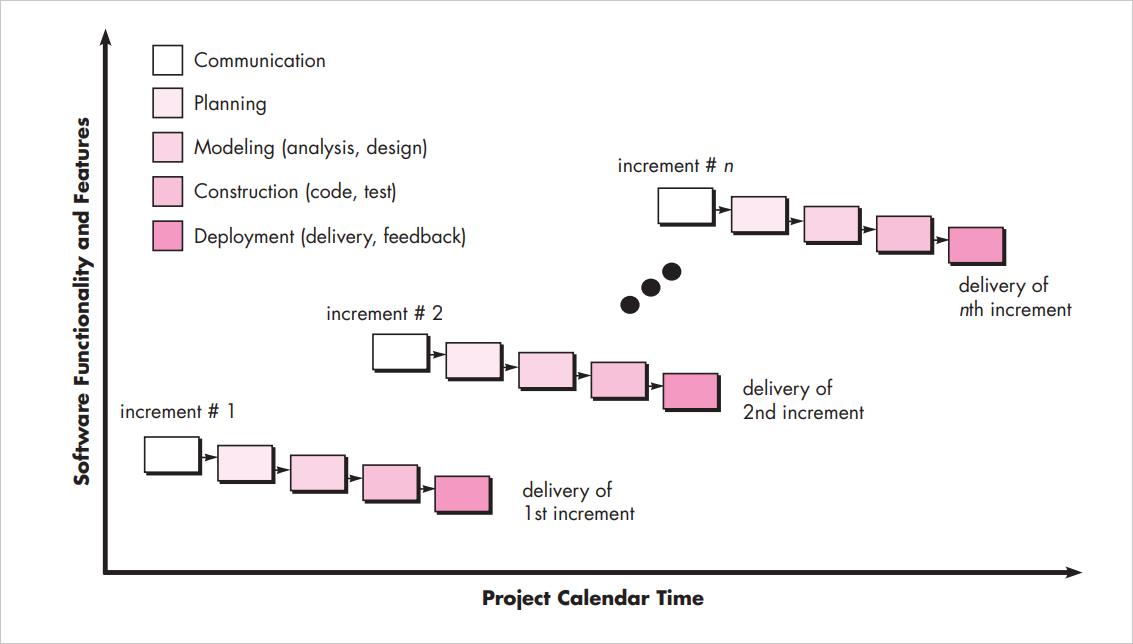
\includegraphics[width=0.8\textwidth]{informatica/ejemplo_modelo_incremental}
    \caption{Ejemplo del modelo de desarrollo incremental. Podemos ver que en cada iteración aplicamos un modelo de desarrollo en cascada. En nuestro caso, cada iteración corresponderá con cada una de las bases de datos sobre las que iteramos. Imagen extraída de \cite{informatica:libro_metodologias_desarrollo}}
\end{figure}

Para cada base de datos sobre la que trabajamos, consideramos las siguientes fases del modelo en cascada para esa iteración:

\begin{itemize}
    \item Análisis: realizamos un análisis exploratorio de la base de datos con la que trabajamos en esta iteración (véase \customref{isec:base_datos_usada}). Estudiamos las técnicas que queremos aplicar y nos marcamos una serie de objetivos para esta iteración
    \item Diseño: en base al estudio realizado sobre el \textit{dataset} y las técnicas que queremos aplicar, definimos qué módulos de código debemos de introducir, qué interfaces deben cumplir para interactuar con otros módulos de código, las propiedades que queremos verificar en los \textit{tests}, distintos \textit{pipelines} que seguir en la experimentación...
    \item Implementación: desarrollamos el código necesario para cumplir con el diseño realizado previamente. En esta fase también incluimos el desarrollo de \textit{tests} para realizar las validaciones
    \item Optimización: en esta fase realizamos \textit{profiles} para detectar partes críticas del código, introducimos \textit{benchmarks} para estudiar el impacto de los cambios realizados, y llevamos a cabo dichos cambios. Esto se explica en detalle en \customref{isec:optimizacion_codigo}. Esta fase es opcional, no se realiza salvo que en la iteración se detecten problemas de rendimiento relevantes
    \item Experimentación: lanzamos los \textit{pipelines} desarrollados en la fase anterior (véase \customref{isec:pipeline}), analizamos los resultados obtenidos, buscamos anomalías en el proceso o en los resultados, ... Esta fase es fundamental a la hora de marcar los objetivos y problemas a resolver en la siguiente iteración sobre una nueva base de datos
\end{itemize}

Para organizar todas las tareas de cada iteración, que nacen en las fases de análisis, diseño e implementación, usamos la \textbf{metodología \textit{Kanban}} \cite{informatica:kanban_paper}. En dicha metodología se usa un tablero, en el que tarjetas que representan tareas a realizar se colocan sobre columnas que representan distintos estados. Usamos cuatro estados:

\begin{itemize}
    \item \textit{Backlog} o tareas que no sabemos si vamos a llevar a cabo
    \item \textit{To-do} o tareas que debemos llevar a cabo.
    \item \textit{In-progress} o tareas que actualmente estamos trabajando
    \item \textit{Done} o tareas que ya se han completado
\end{itemize}

Esto permite tener una visualización rápida del estado de la iteración. Como comentaremos detalladamente en \customref{isec:github_buenas_practicas}, usaremos la utilidad de proyectos que ofrece \textit{Github} para tener acceso a un tablero \textit{kanban}. En la siguiente imagen se muestra un ejemplo del estado de este tablero:

\begin{figure}[H]
    \centering
    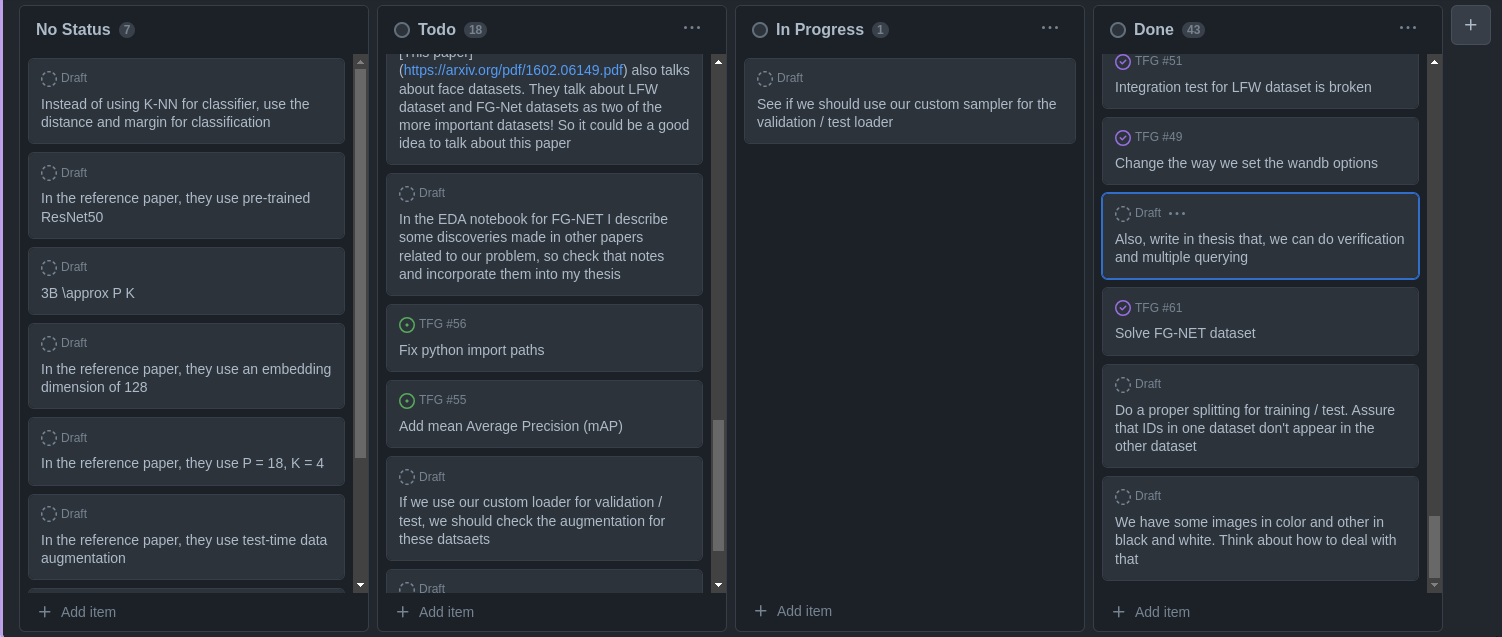
\includegraphics[width=0.9\textwidth]{informatica/kanban_board}
    \caption{Ejemplo del estado de nuestro tablero \textit{kanban} en un momento concreto durante la fase de desarrollo. Podemos ver las cuatro columnas que ya hemos descrito. \textit{Github} le da el nombre \textit{No Status} a la columna que nosotros usamos como \textit{backlog}}
\end{figure}

Comenzamos a desarrollar el proyecto en Febrero de 2022. Sabemos que, debido a los exámenes universitarios, apenas trabajaremos en los meses de Enero, Mayo y Junio. Por tanto, consideraremos que en estos meses no trabajemos ninguna hora (aunque en la práctica sí que consigamos sacar algo de tiempo). Los meses en los que más trabajaremos serán Febrero, Julio, Agosto y Septiembre. En estos meses tenemos previsto trabajar al menos 20 horas semanales. En el resto de meses consideramos que trabaremos al menos 2 horas semanales. Por tanto, en los dos años que dedicamos al proyecto de informática, dedicaremos al menos 720 horas.

Teniendo todo esto en cuenta, inicialmente planificamos el proyecto tal y como describe el siguiente diagrama de Gannt:

\begin{figure}[H]
    \centering
    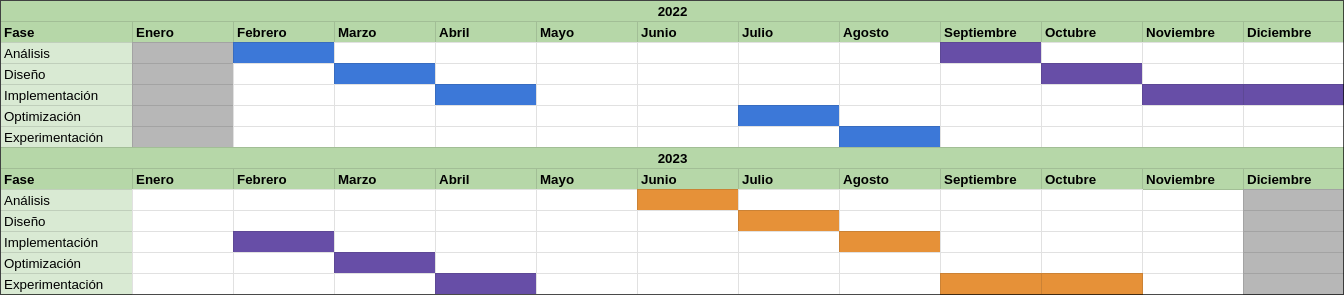
\includegraphics[width=1.0\textwidth]{informatica/diagrama_gannt_ideal}
    \caption{Diagrama de \textit{Gantt} que describe la planificación original del proyecto. El color azul corresponde al \textit{dataset} \textit{MNIST}. El color morado corresponde al \textit{dataset} \textit{LFW}. El color naranja corresponde a los \textit{datasets} \textit{FG-Net} junto con \textit{CACD}}
\end{figure}

Sin embargo, por los problemas enfrentados durante el desarrollo, y por inexactitudes en la planificación, acabamos distribuyendo el tiempo dedicado al trabajo tal y como se muestra en el siguiente diagrama de Gannt:

\begin{figure}[H]
    \centering
    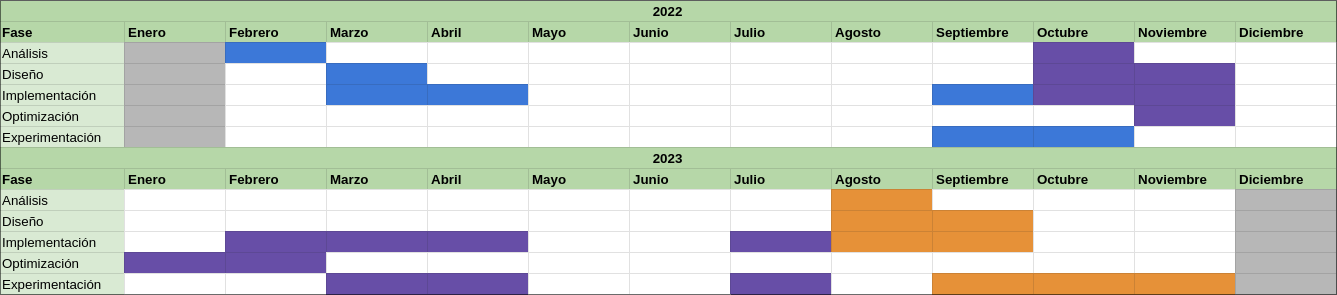
\includegraphics[width=1.0\textwidth]{informatica/diagrama_gannt_real}
    \caption{Diagrama de \textit{Gantt} que describe la distribución real del tiempo dedicado al proyecto. Seguimos el mismo código de colores que en el diagrama anterior}
    \label{img:gannt_real}
\end{figure}

En el repositorio abierto de \textit{Github} \cite{informatica:repogithub} donde hemos desarrollado el proyecto, podemos verificar los tiempos que aparecen en \customref{img:gannt_real}.

En cuanto a la planificación económica, tenemos en cuenta los siguientes aspectos:

\begin{itemize}
    \item El salario aproximado de un investigador en Ciencia de Datos y Aprendizaje Automático es de 35 €/h. Teniendo en cuenta que hemos dedicado al menos 720 horas de trabajo, esto supone un coste de 25.200€
    \item El valor del ordenador que hemos usado para trabajar: 600€
    \item El valor de los servidores \textit{nGPU} donde se han lanzado los procesos (véase \customref{isec:entorno_ejecucion}). Se estima un coste de unos 145€ semanales. Teniendo en cuenta que hemos tenido acceso desde Marzo de 2023, y usamos estos servidores hasta Octubre de 2023, esto supone un coste de 4.640€
\end{itemize}

Todo esto supone un \textbf{coste total} de unos 30.440€.
